\documentclass{article}
\usepackage{hyperref}
\usepackage[procnames]{listings}
\usepackage{color}
\title{Assignment 4}
\date{2016-02-25}
\author{Tarek Fouda}
\usepackage[pdftex]{graphicx}
\usepackage{listings}
\usepackage{alltt}

\definecolor{dkgreen}{rgb}{0,0.6,0}
\definecolor{gray}{rgb}{0.5,0.5,0.5}
\definecolor{mauve}{rgb}{0.58,0,0.82}

\lstset{
	basicstyle=\footnotesize,
	breaklines=true,
}

\begin{document}
  \maketitle
\section{Introduction}
This report explains how I managed to solve Assignment 4  in Web Science class which is due 02/25/2016. It is mainly consisted of Two Questions and two extra credit points questions. Will show my approaches and implementation in each of the two Questions.

\section{Problem 1 Getting the Median/Standard Deviation/Mean} \label{problem1}

\subsection{friendship paradox}

Basically, there is something called the ``friendship paradox''  which checks if your friends have more friends than you have.
First, I implemented a program that takes the xml file given in the assignment, and extract all the data tags that has a key equals to `` Friends count'' and put it in a text file named ``friendscount.txt''. 
We were looking to the following tag:
\begin{lstlisting}
<data key="friend_count">
\end{lstlisting} 

The following program is the code that performs this extraction from the xml file:
\lstinputlisting[language=Python,frame=single,caption={python code to get friend counts from XML file},label=lst:q2code1,captionpos=b,numbers=left,
numberstyle=\tiny\color{gray},
  keywordstyle=\color{blue},
  commentstyle=\color{dkgreen},
  stringstyle=\color{mauve},showspaces=false,showstringspaces=false,basicstyle=\footnotesize]{extractingxml.py}

After that we get the text file named ``friendscount.txt'' and we loop through all it's lines and get the number that exists in each line. That will be the number of friends.
The following is the program that performs such a task:
\lstinputlisting[language=Python,frame=single,caption={python code to get number in each line},label=lst:q2code1,captionpos=b,numbers=left,
numberstyle=\tiny\color{gray},
  keywordstyle=\color{blue},
  commentstyle=\color{dkgreen},
  stringstyle=\color{mauve},showspaces=false,showstringspaces=false,basicstyle=\footnotesize]{num.py}

The next step after getting the number of friends is to perform the calculations to get the mean, standard deviation, and median of the number of friends that the professor's friends have.
\lstinputlisting[language=Python,frame=single,caption={python code to get number in each line},label=lst:q2code1,captionpos=b,numbers=left,
numberstyle=\tiny\color{gray},
  keywordstyle=\color{blue},
  commentstyle=\color{dkgreen},
  stringstyle=\color{mauve},showspaces=false,showstringspaces=false,basicstyle=\footnotesize]{q1.py}

The following is the graph, the x-co-ordinates represents the friends number, and the y-co-ordinates represent the number of friends the professor's friends have.

\begin{figure}
\centering
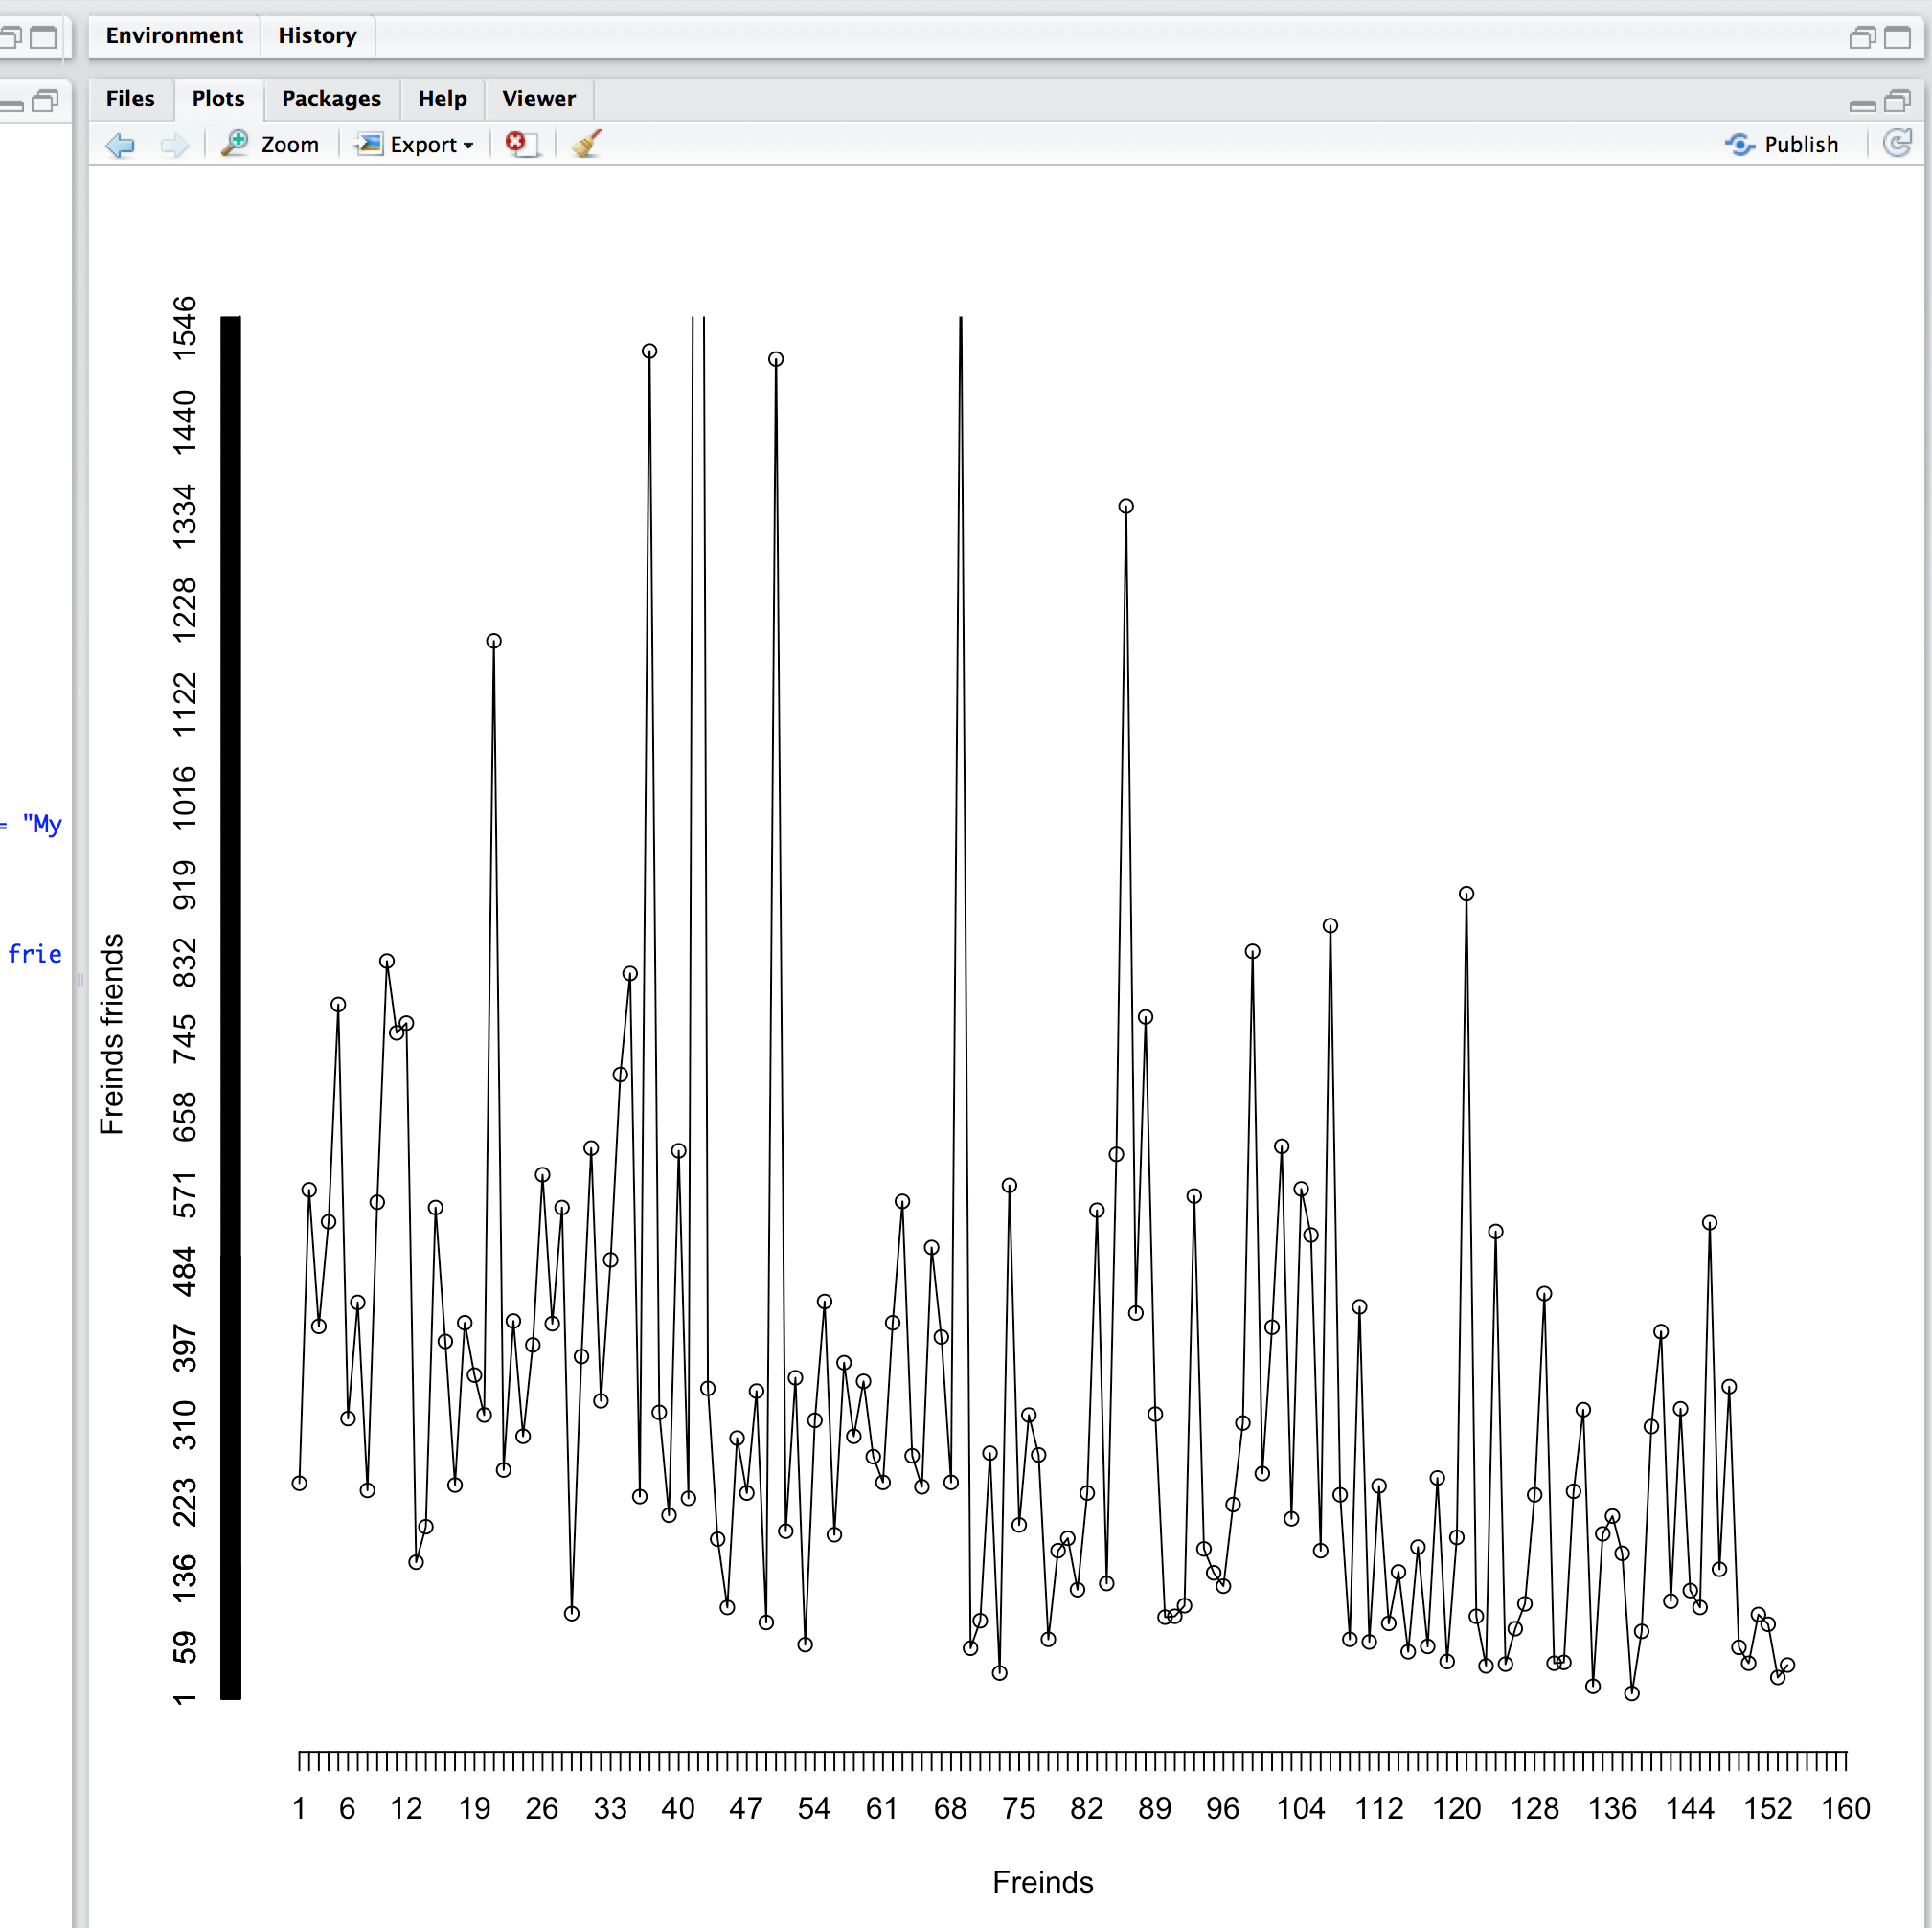
\includegraphics[scale=0.25]{fig1.png}
\caption{TheGraph}
\label{fig:fig.png}
\end{figure}

The calculations which were used in the above graph are shown below upon executing the python code:

\begin{figure}
\centering
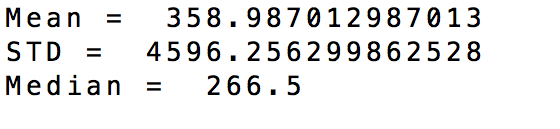
\includegraphics[scale=0.95]{ah.png}
\caption{TheGraph}
\label{fig:fig.png}
\end{figure}
\newpage


\section{Problem number 2}
In thisPart of the assignment we were required to get the number of followers my twitter account has and see if the ``friendship paradox'' will hold, or in other words if my followers have more followers than I have.

So we need to check the number of followers I have, then loop on each one of these followers, and check the number of followers they have and do the calculations the same as part 1.

I used Tweepy Api to get the number of followers. 

\lstinputlisting[language=Python,frame=single,caption={python code to get number of followers my twitter username and my follower's usernames have},label=lst:q2code1,captionpos=b,numbers=left,
numberstyle=\tiny\color{gray},
  keywordstyle=\color{blue},
  commentstyle=\color{dkgreen},
  stringstyle=\color{mauve},showspaces=false,showstringspaces=false,basicstyle=\footnotesize]{followers.py}

And this is a sample of the output I get on running the above code:
\begin{figure}
\centering
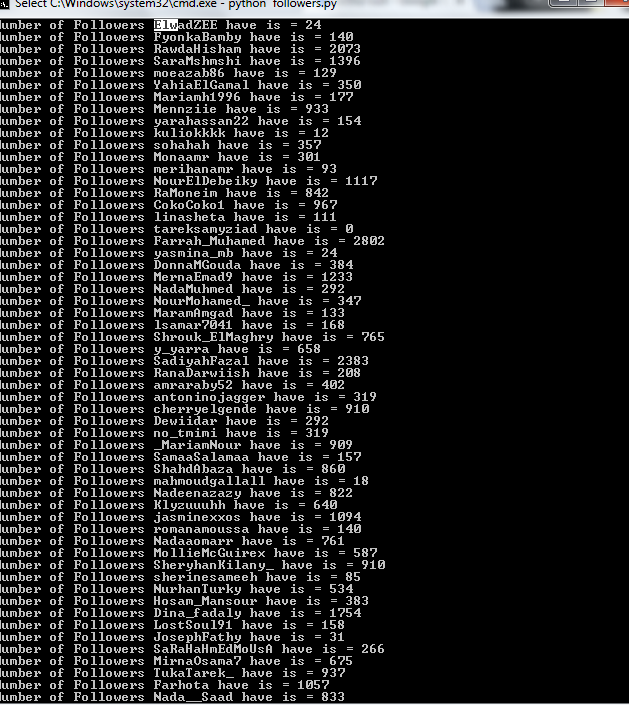
\includegraphics[scale=0.95]{pic3.png}
\caption{The followers and the number of followers they have}
\label{fig:fig.png}
\end{figure}

I printed the output in a text file and by executing the same methods and techniques in \ref{problem1}, I managed to calculate the mean, median and standard deviation. These were the calculations and the graph:

\begin{figure}
\centering
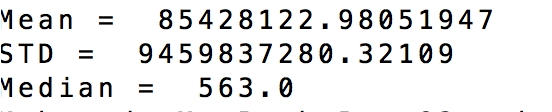
\includegraphics[scale=0.95]{fig2.png}
\caption{The followers and the number of followers they have}
\label{fig:fig.png}
\end{figure}

\begin{figure}
\centering
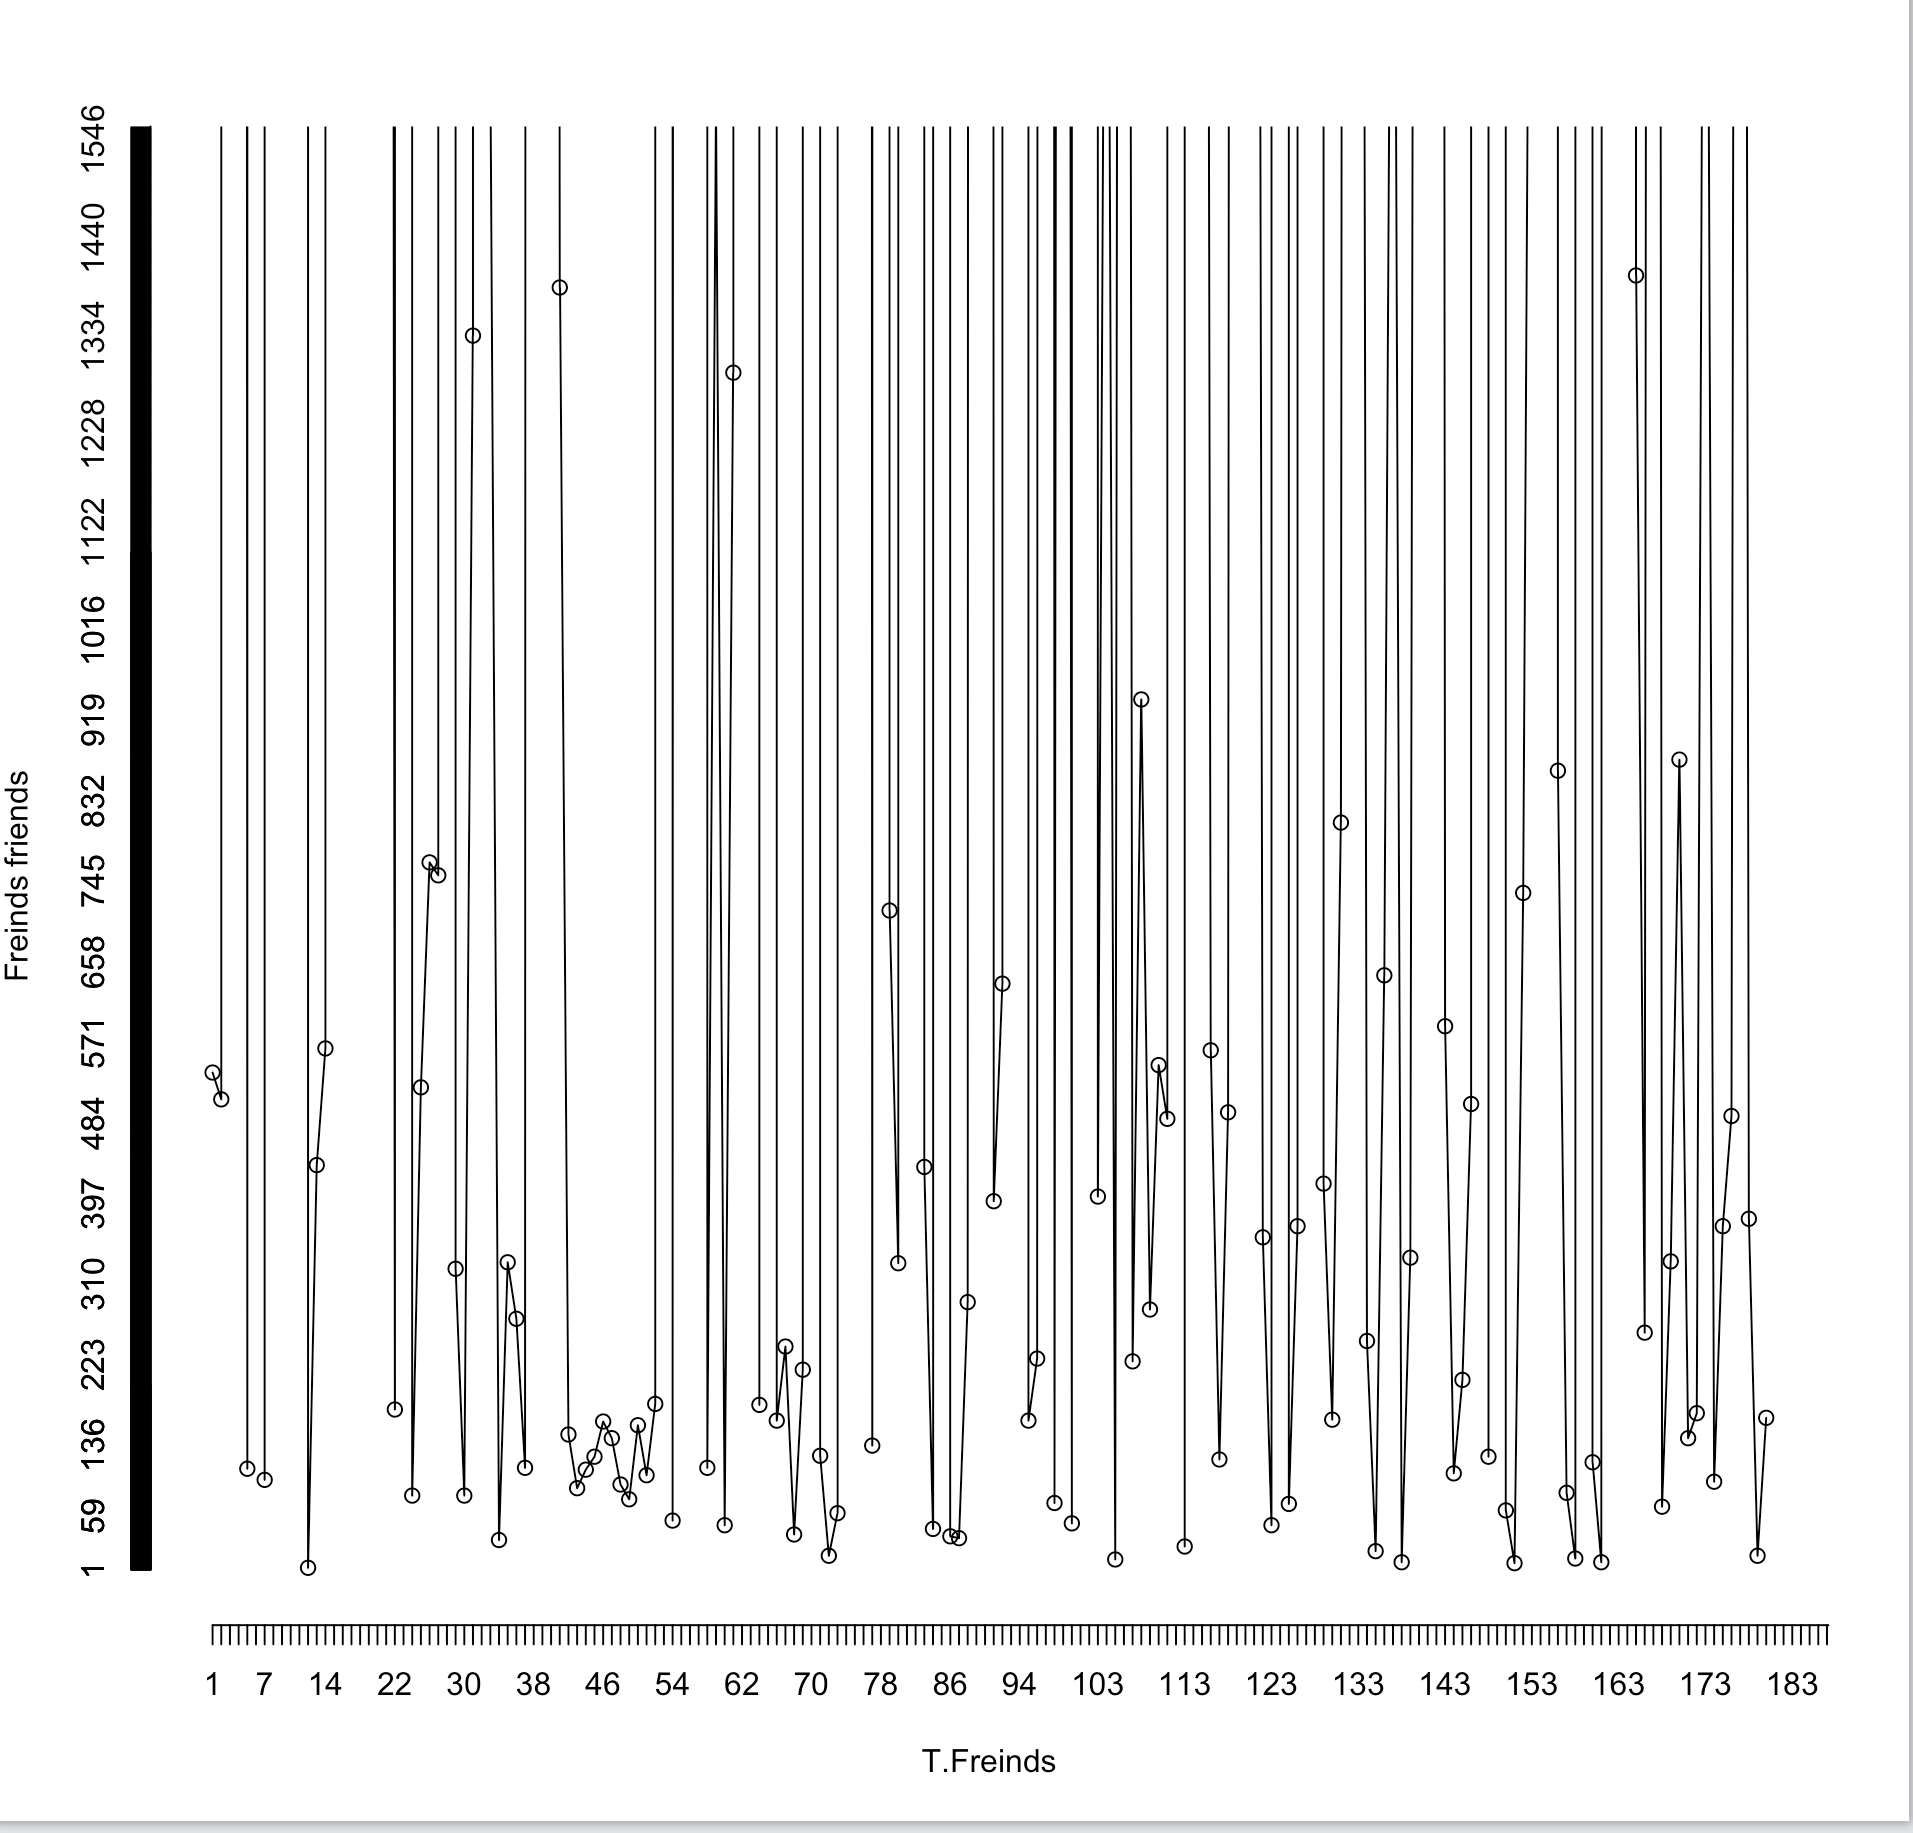
\includegraphics[scale=0.25]{last.png}
\caption{The followers and the number of followers they have}
\label{fig:fig.png}
\end{figure}

So the x-axis has the number of friends I have, and the Y-axis has the number of friends each follower have.
\end{document}